
迁移包含大量库和多个可执行文件的大型项目可能是一个相当大的挑战,这些项目实际上可能是多个层次嵌套的项目,具有一个或多个将多个子项目拉在一起的根项目,而这些根项目本身又包含或需要多个子项目。根据软件组合的大小和复杂性,许多共享公共子项目的根项目可能并排存在,这可能使迁移复杂化。创建项目和子项目的依赖关系图(如下图所示),通常可以帮助我们弄清楚迁移的顺序。每个项目本身可能包含多个项目或目标,这些项目或目标有自己的依赖项:

\begin{center}
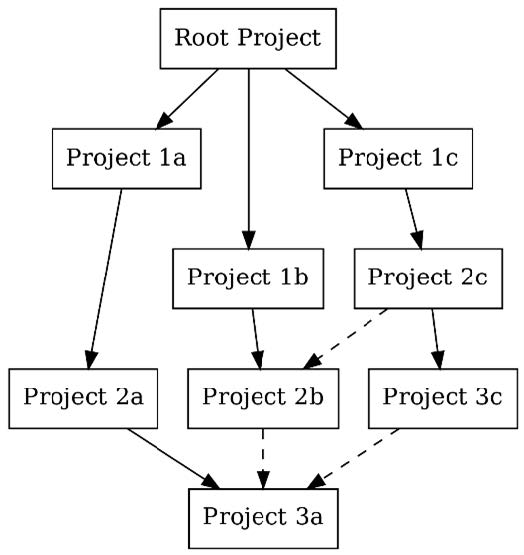
\includegraphics[width=0.3\textwidth]{content/3/chapter15/images/1.jpg}\\
图15.1 显示各种依赖关系的示例项目层次结构
\end{center}

迁移之前,要做的第一件事是彻底分析项目之间如何相互依赖,以及需要以什么顺序构建。根据项目的状态,最终的图可能会非常大,所以确定从哪里开始可能会有点困难。实际上,依赖图往往不像本书中展示的那样简洁。先理清项目脉络,再迁移到CMake,还是先迁移到CMake再理清项目脉络更容易,这取决于实际情况。若项目非常大且复杂,那么首先在图中找到尽可能独立的孤岛,并从那里开始着手。

对于复杂的、分层的项目,有两种迁移策略。一种是自顶向下的方法,首先迁移并替换根项目,然后根据哪个项目具有最少的依赖关系对子项目进行排序。第二种是自底向上的方法,从依赖项最多的项目开始,逐个迁移各个项目。

自顶向下的方法有一个好处,确保完整的项目可以在早期用CMake进行构建、测试和打包,但要求现有的构建系统使用\texttt{ExternalProject}的方式集成到CMake中。自上而下的方法的缺点可能是,早期会生成的CMake项目包含大量自定义代码,用于使用旧系统构建的包。实践中,使用一些临时方法在构建中,包含现有项目是相对快速地获得良好结果的实用方法,并且在一定程度上减轻了为相同子项目维护两个构建系统的工作量。

自底向上方法的好处是:每个库迁移到CMake已经迁移可以使用依赖项。缺点是只有在所有子项目都能用CMake构建后,根项目才能替换。即使项目从下往上迁移,好的做法是尽早创建根CMake项目,与原始构建系统中的根项目同时存在。这就可以尽早在新的CMake项目中放入外部依赖项、安装配置和打包说明。

下面的图表说明了自顶向下和自底向上策略是如何同时出现的。方框旁边的数字表示迁移的顺序:

\begin{center}
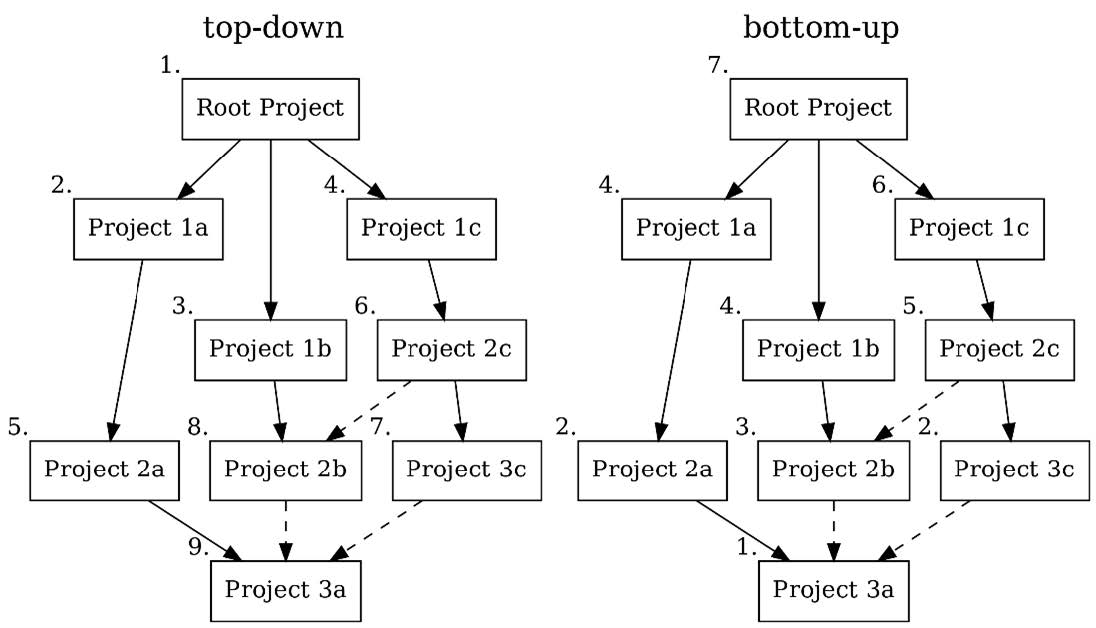
\includegraphics[width=0.8\textwidth]{content/3/chapter15/images/2.jpg}\\
图15.2 迁移顺序的示例
\end{center}

除了整体的迁移策略之外,另一件需要考虑的事情是项目是要设置为超级构建,还是常规项目。当使用自顶向下的方法时,超级构建结构可能更容易迁移,因为好处是更容易通过设计集成非CMake项目。

无论选择自顶向下的方法,还是自底向上的方法来迁移单个项目,迁移大型项目的策略看起来都有以下几点:

\begin{enumerate}
\item 
分析依赖关系、项目层次结构和部署单元是什么。

\item 
决定迁移策略,以及是使用常规项目结构,还是超级构建。

\item 
创建或迁移根项目,并使用\texttt{ExternalProject}、\texttt{FetchContent}或中间查找模块(若使用二进制包)拉入所有尚未转换的项目。

\item
使用CMake处理项目级别的依赖关系。

\item
如本章最后一节所述,将子项目逐个地转换为CMake。若使用中间查找模块,则逐个替换:

\begin{enumerate}[label=\roman*]
\item
可以将依赖项处理更改为包管理器。

\item
找到常用选项,并将它们传递至根目录并创建预设。
\end{enumerate}

\item
迁移子节点时,若还没有完成,可以在CMake中使用该子节点的已打包文件。

\item
清理、重新组织文件和项目、提高性能等。
\end{enumerate}

通过分析现有的项目层次结构和依赖关系来开始迁移,这将帮助您建立一个迁移计划,以便与所有相关人员进行沟通。创建可视化关系图通常是一个很好的方式,尽管对于非常大的项目,这本身就可能成为一个相当大的挑战。创建迁移计划时要牢记的另一个要点是,确定什么是通常部署在一起,以及哪个子项目有哪个发布频率。很少更改和发布的项目对于迁移来说,可能不像那些经常修改和发布的项目那么重要,确定部署单元与如何打包项目密切相关。根据组织方式的不同,在所有项目迁移之前,可能无法将打包迁移到CMake。

我们主要讨论了子项目,但在分析现有结构时,重要的是要认识到哪些子项目实际上是可以作为独立的项目,在整个项目上下文中构建的项目;哪些子项目可以作为常规的CMake目标来处理,而很少在项目上下文中构建。

创建CMakeLists.txt主文件将涵盖基本的项目设置,并包括必要的模块,如FetchContent、CTest、CPack等。虽然不是直接在CMakeLists.txt文件中,但也可以在这里设置工具链文件、构建容器或用于交叉编译的sysroot。对于大型项目,主CMakeLists.txt通常不直接包含目标。相反,可将它们包含在\texttt{add\_subdirectory}或\texttt{FetchContent}中,或者\texttt{ExternalProject}的超级构建中。主CMakeLists.txt应该有以下的结构:

\begin{enumerate}
\item 
项目定义和CMake的最低版本。

\item
全局属性和默认变量,如最低语言标准、自定义构建类型以及搜索和模块路径。

\item
项目范围内使用的模块和辅助函数。

\item
通过\texttt{find\_package()}包含的项目范围的外部依赖项。

\item
构建目标和子项目,使用\texttt{add\_subdirectory}、\texttt{FetchContent}添加,或者在超构建下使用\texttt{ExternalProject}。

\item
整个项目的测试,每个子项目都有自己的单元测试,但是集成或系统测试可能位于顶层。

\item
CPack的包装说明。
\end{enumerate}

根据定义的复杂性,将外部依赖项的处理、测试和打包放到自己的子目录中,可能有助于保持CMake文件的简短和简洁。整个项目使用的外部依赖可能是大型软件框架,如Qt或Boost,也可能是小型但经常使用的实用工具库。

对于自顶向下的方法,可以一开始导入子项目,然后逐个迁移。当使用自底向上策略时,构建目标和子项目很可能为空,然后随着项目的迁移而填充。迁移子项目时,要留意可以传递到根项目,或到预设的公共依赖项或构建选项。

迁移了所有的子项目,仍然有一些维护任务,例如组织打包、交付和分组测试。此外,在迁移所有内容后,CMake文件中仍有一些混乱也实属正常,因此需要再进行一轮清理,确保迁移项目的功能已经处于可用状态。

迁移大型项目是一项挑战,特别是当构建过程很复杂且缺乏文档时。软件的构建方式有很多种,本节描述的策略试图给出一种通用的方法。然而,每个迁移都有自己独特的方式。某些情况下,构建系统非常复杂,前面描述的迁移策略非但没有帮助,反而起到了反作用。例如,将未迁移的项目包含到CMake中非常困难,因此逐步迁移可能比从头开始构建更费力。让我们来了解一下,在使用自顶向下的方法开始时,如何包含使用原始构建系统的子项目。

\subsubsubsection{15.4.1\hspace{0.2cm}自顶向下迁移时集成历史遗留项目}

对于自顶向下的迁移策略,现有的项目在一开始就提供给CMake。最简单的方法是使用\texttt{ExternalProject},不管是否打算进行超级构建。导入的目标可以直接定义,也可以使用find模块定义。对于常规项目,这只是一个中间步骤,以便能够相对快速地构建完整的项目,并将配置和构建顺序的控制权移交给CMake。生成的CMake代码可能不是特别友好,但第一个目标是使用CMake构建根项目。在迁移子项目时,一定要一步步地清理。对于由多个库组成的普通项目,或者通过Git子模块或类似的方式引入依赖项的项目,\texttt{ExternalProject\_Add}会省略下载,而是指定SOURCE\_DIR属性。包含Autotools项目的CMake代码可能如下所示:

\begin{lstlisting}[style=styleCMake]
include(ExternalProject)
set(ExtInstallDir ${CMAKE_CURRENT_BINARY_DIR}/install)
ExternalProject_Add(SubProjectXYZ_ext
	SOURCE_DIR ${CMAKE_CURRENT_LIST_DIR}/SubProjectXYZ/
	INSTALL_DIR ${ExtInstallDir}
	CONFIGURE_COMMAND <SOURCE_DIR>/configure --prefix <INSTALL_DIR>
	INSTALL_COMMAND make install
	BUILD_COMMAND make
)
add_library(SubProjectXYZ::SubProjectXYZ IMPORTED SHARED)
set_target_properties(SubProjectXYZ::SubProjectXYZ
	PROPERTIES IMPORTED_LOCATION
		"${CMAKE_CURRENT_LIST_DIR}/SubProjectXYZ/lib/libSubProjectXYZ.so"
	INTERFACE_INCLUDE_DIRECTORIES
		"${CMAKE_CURRENT_LIST_DIR}/SubProjectXYZ/include"
	
	IMPORTED_LINK_INTERFACE_LANGUAGES "CXX"
)
...
add_dependencies(SomeTarget SubProjectXZY_ext)
target_link_libraries(SomeTarget SubProjectXYZ::SubProjectXYZ)
\end{lstlisting}

因为\texttt{ExternalProject}只在构建时提供内容,所以这种方法只适用于本地文件夹中可用的子项目。因为包含导入目标的目录,当在\texttt{target\_link\_libraries}中使用时,必须在配置时存在,导出位置应该指向源目录,而不是外部项目的安装位置。

\begin{tcolorbox}[colback=blue!5!white,colframe=blue!75!black,title=临时解决方案]
这里描述的使用\texttt{ExternalProject}和\texttt{FetchContent}是一种临时解决办法,以便在迁移时能够将遗留项目包含在CMake构建中,这些都不是适合在生产环境中使用的良好实践。该模式允许使用原始的构建系统,并将提供一个导入的目标来链接已经迁移的项目。无论创建这种中间项目结构的努力,是否通过能够在早期使用CMake构建完整的项目来证明合理,都必须对每种情况单独考虑。

若从Microsoft Visual Studio迁移而不是使用\texttt{ExternalProject},可以使用\texttt{include\_external\_msproject()}直接包含项目文件。
\end{tcolorbox}


























